\chapter{Конструкторская часть}

В данном разделе представлены схемы алгоритмов для вычисления расстояний Левенштейна и Дамерау~---~Левенштейна.

\section{Разработка алгоритмов}


Алгоритмы получают на вход две строки $S_1$ и $S_2$. 

На рисунке \ref{fig:Liter} представлена схема алгоритма для вычисления расстояния Левенштейна. 
Алгоритм находит оптимальное расстояние между двумя строками, используя динамическое программирование.

\begin{figure}[h]
	\centering
	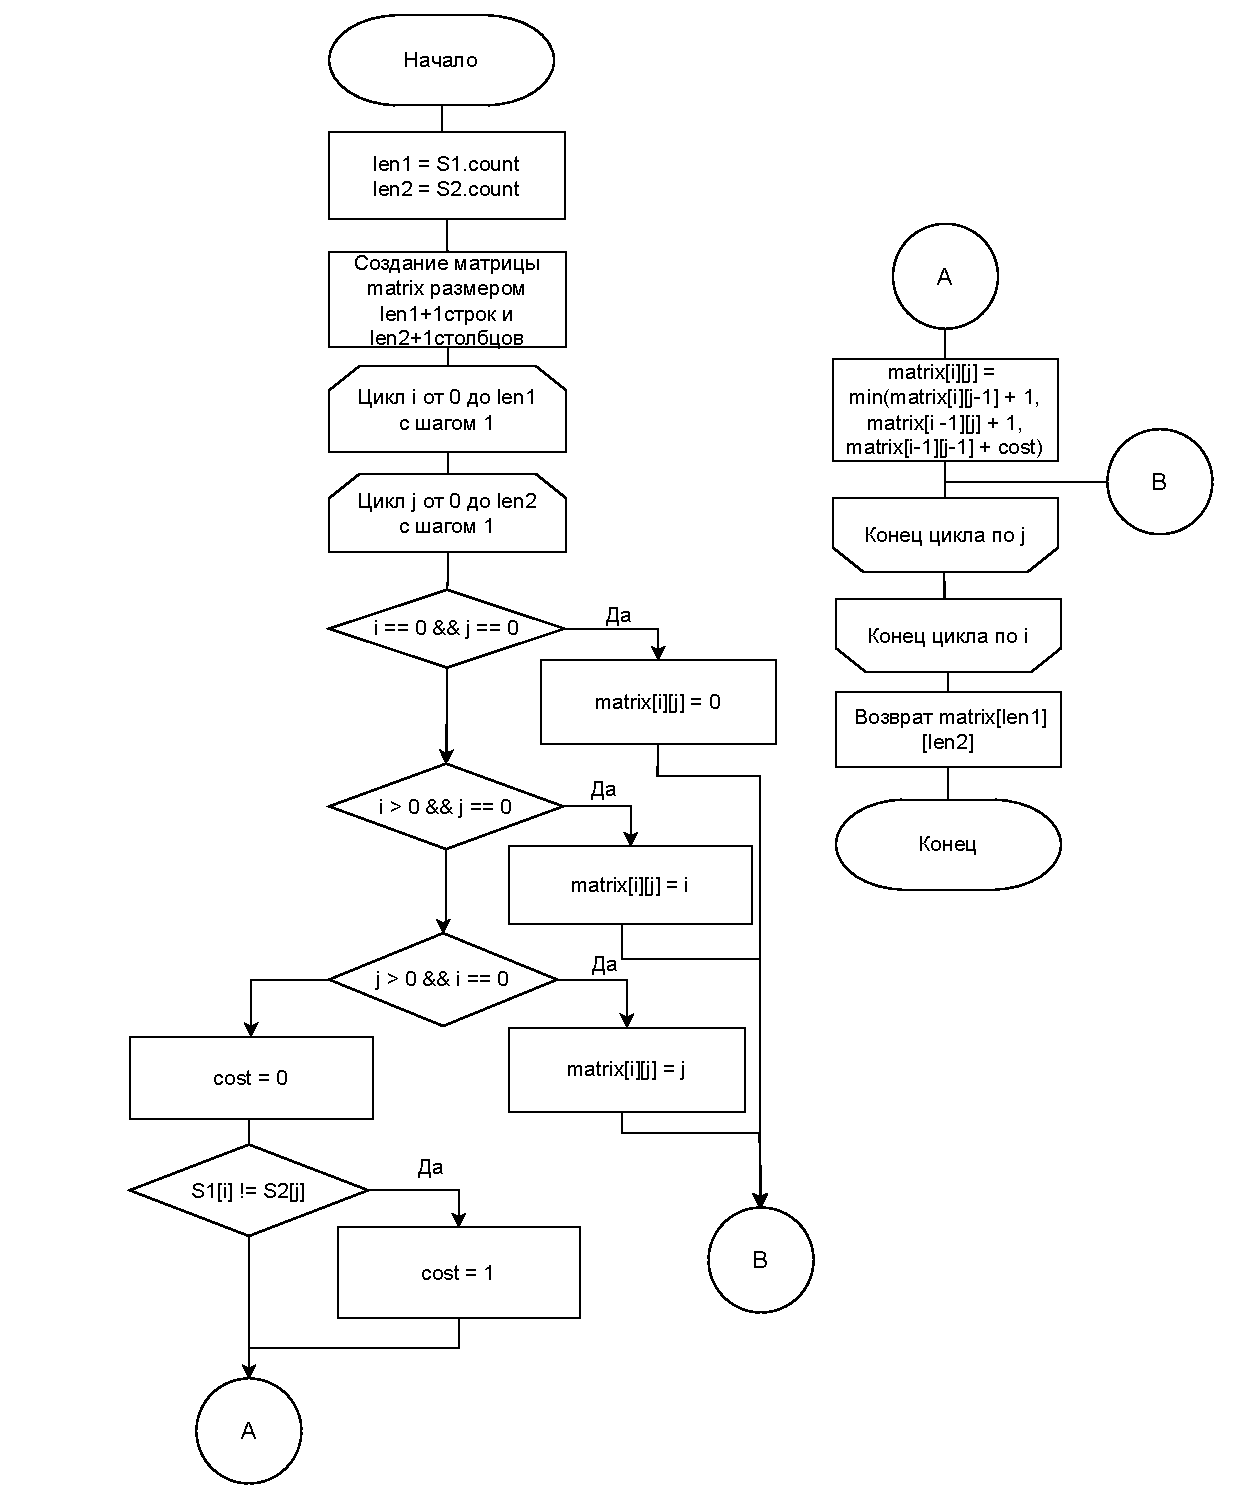
\includegraphics[height=0.8\textheight]{img/levenshtein.pdf}
	\caption{Схема алгоритма для вычисления расстояния Левенштейна}
	\label{fig:Liter}
\end{figure}

На рисунках \ref{fig:DLiter} -- \ref{fig:DLrechash2} представлены схемы алгоритмов для вычисления расстояния Дамерау~---~Левенштейна. 

\begin{figure}[h]
	\centering
	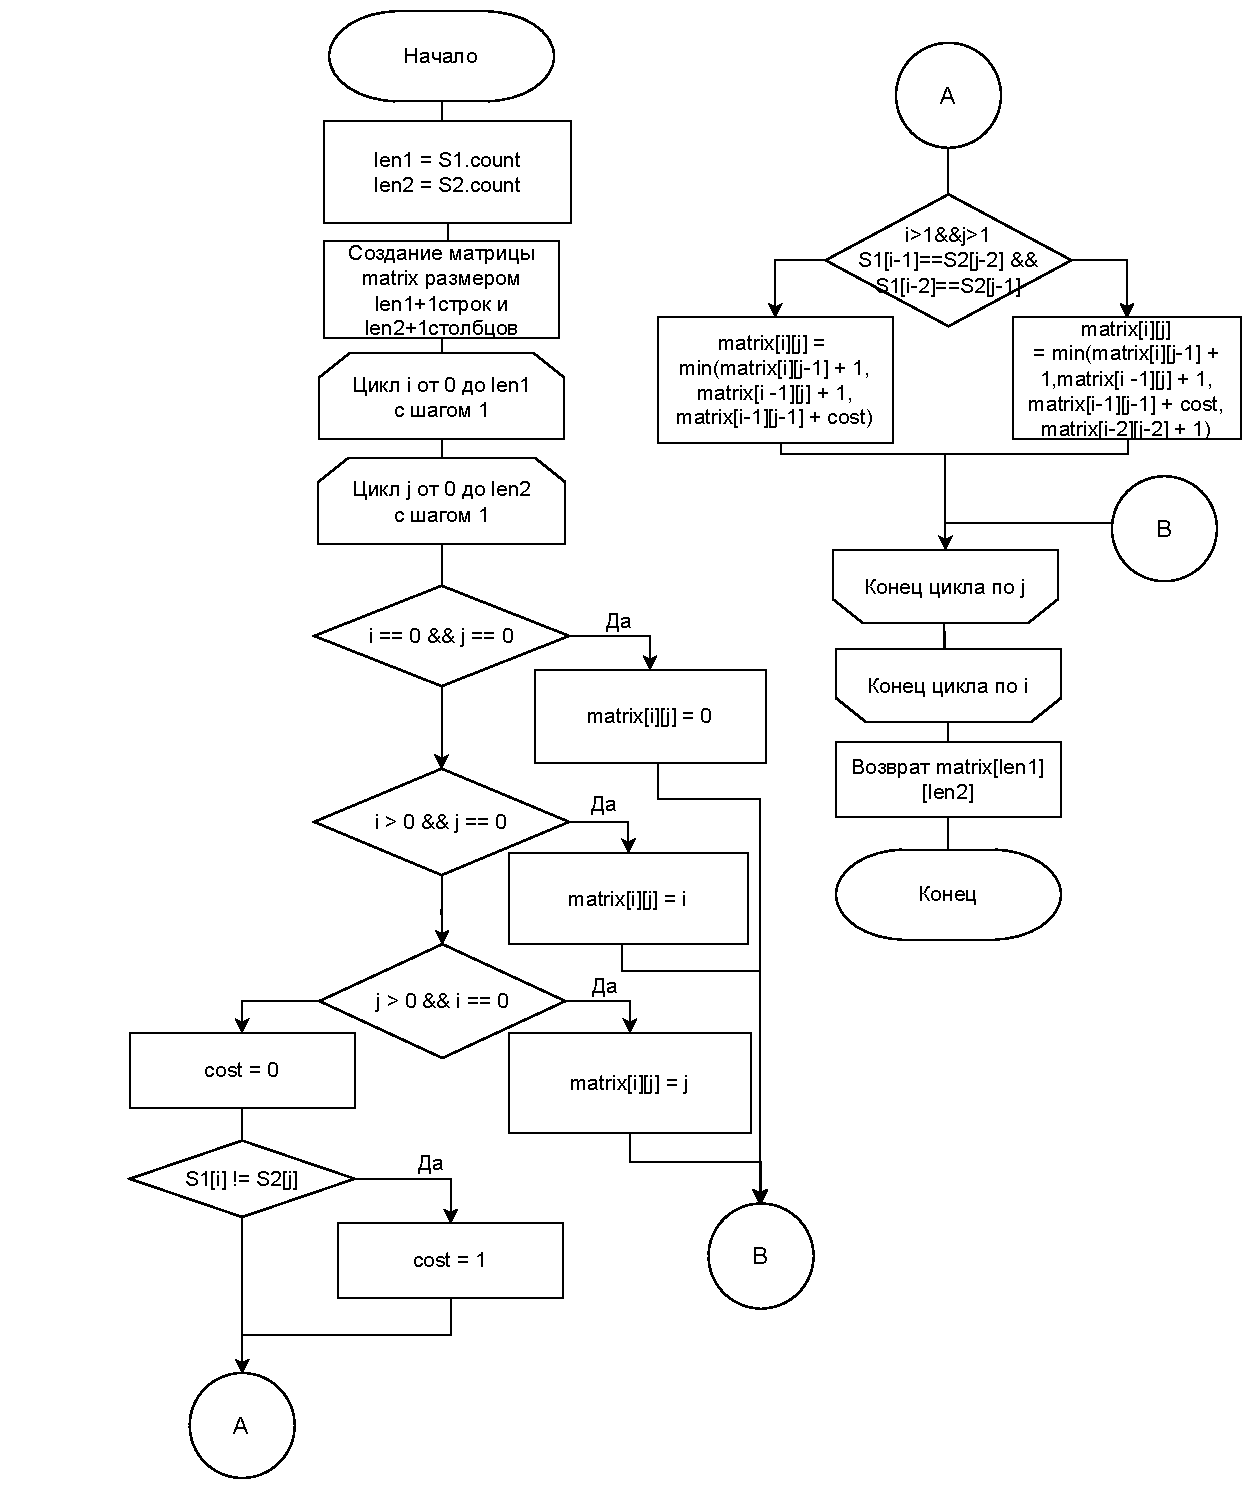
\includegraphics[height=0.8\textheight]{img/DLevenshtein.pdf}
	\caption{Схема алгоритма для вычисления расстояния Дамерау~---~Левенштейна}
	\label{fig:DLiter}
\end{figure}

\clearpage

\begin{figure}[h]
	\centering
	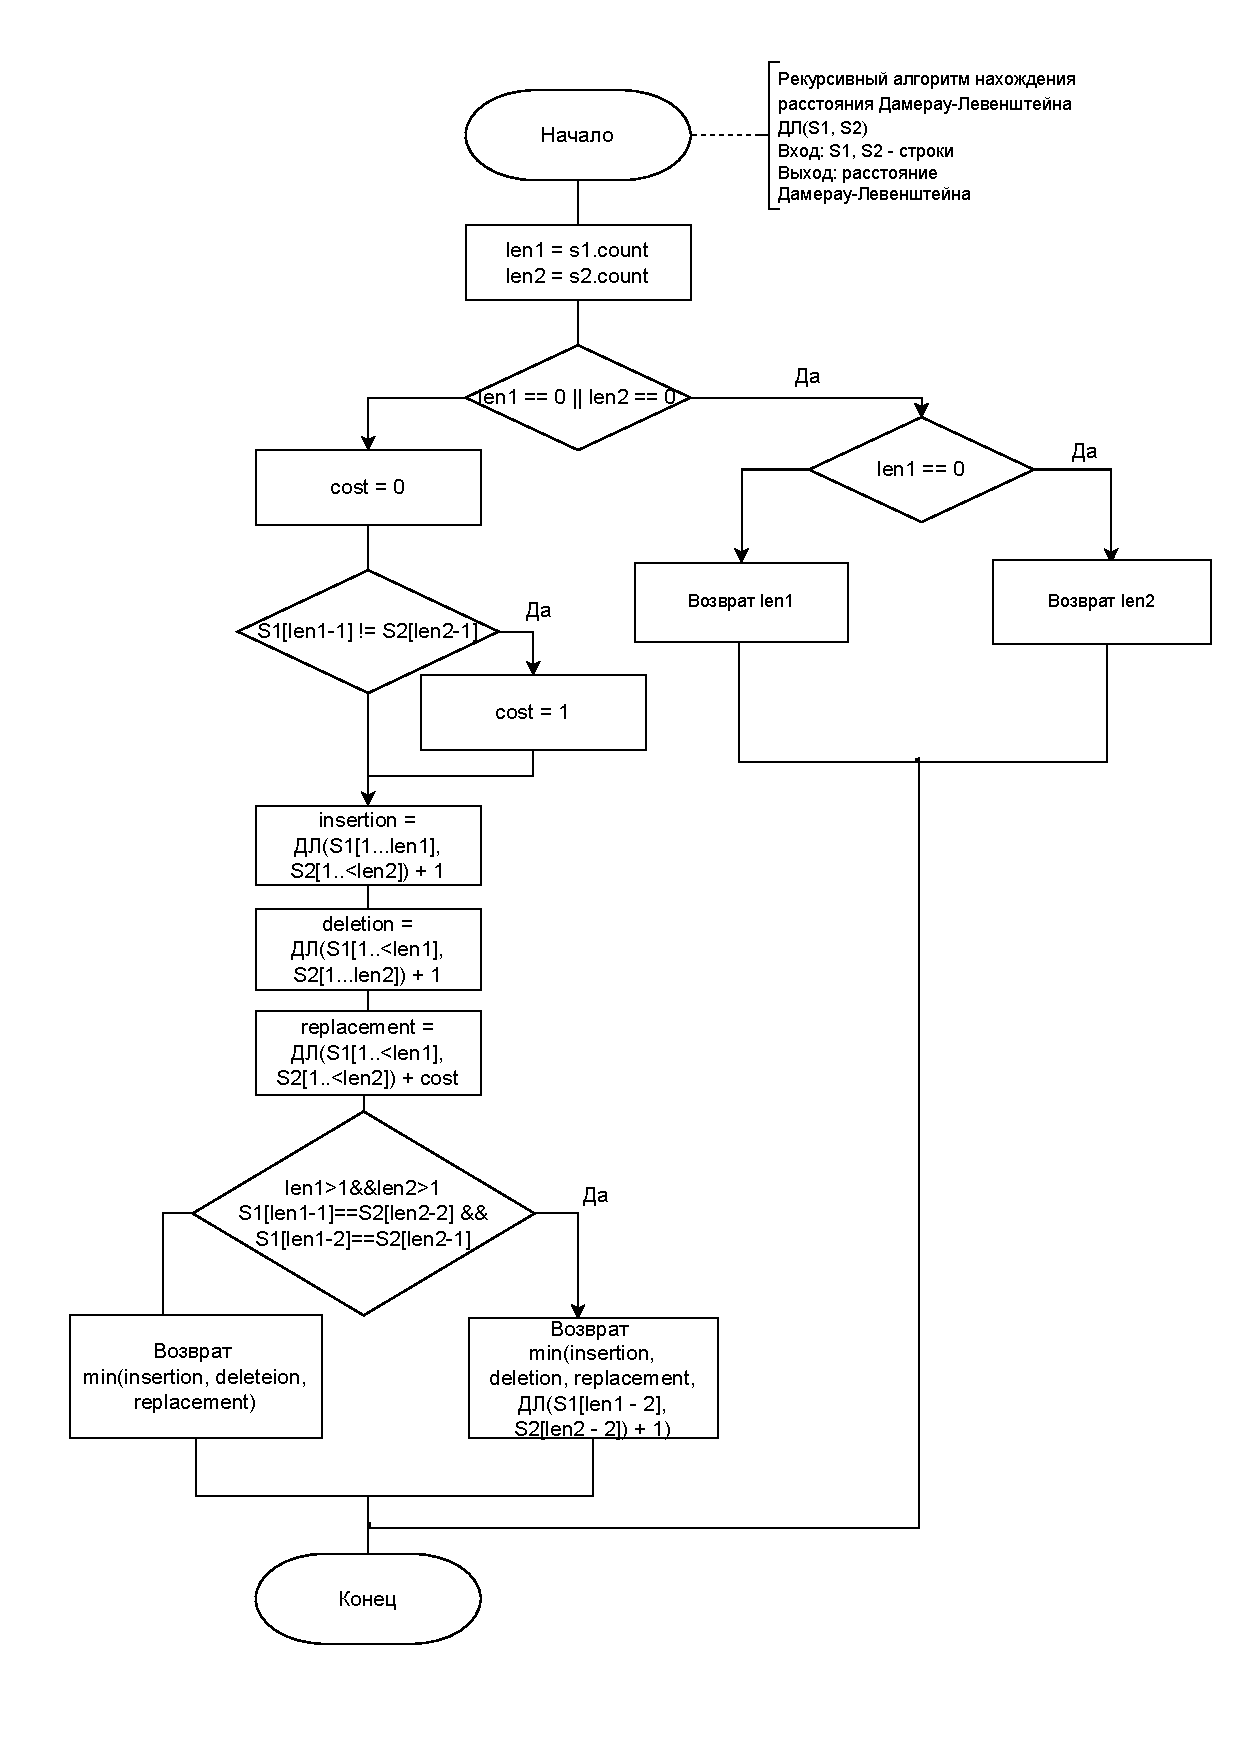
\includegraphics[height=0.8\textheight]{img/recursiveDLevenshtein.pdf}
	\caption{Схема рекурсивного алгоритма для вычисления расстояния Дамерау~---~Левенштейна}
	\label{fig:DLrec}
\end{figure}

\clearpage

\begin{figure}[h]
	\centering
	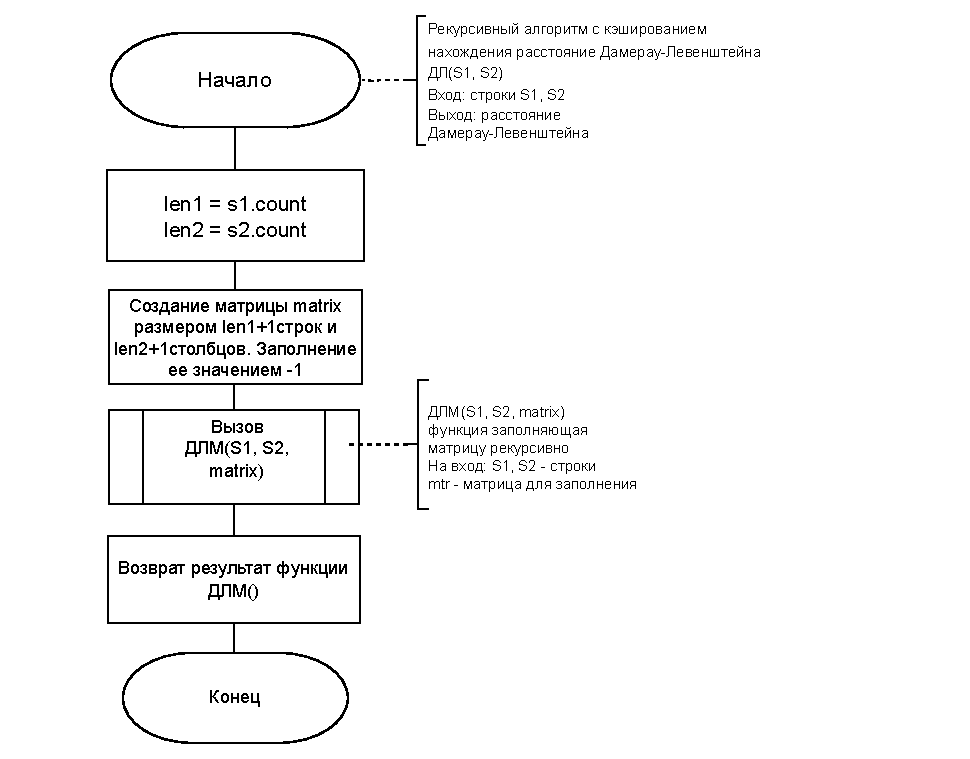
\includegraphics[height=0.6\textheight]{img/recursiveCacheDLevenshtein1.pdf}
	\caption{Схема рекурсивного алгоритма для вычисления расстояния Дамерау~---~Левенштейна с использованием кэша}
	\label{fig:DLrechash1}
\end{figure}

\clearpage

\begin{figure}[h]
	\centering
	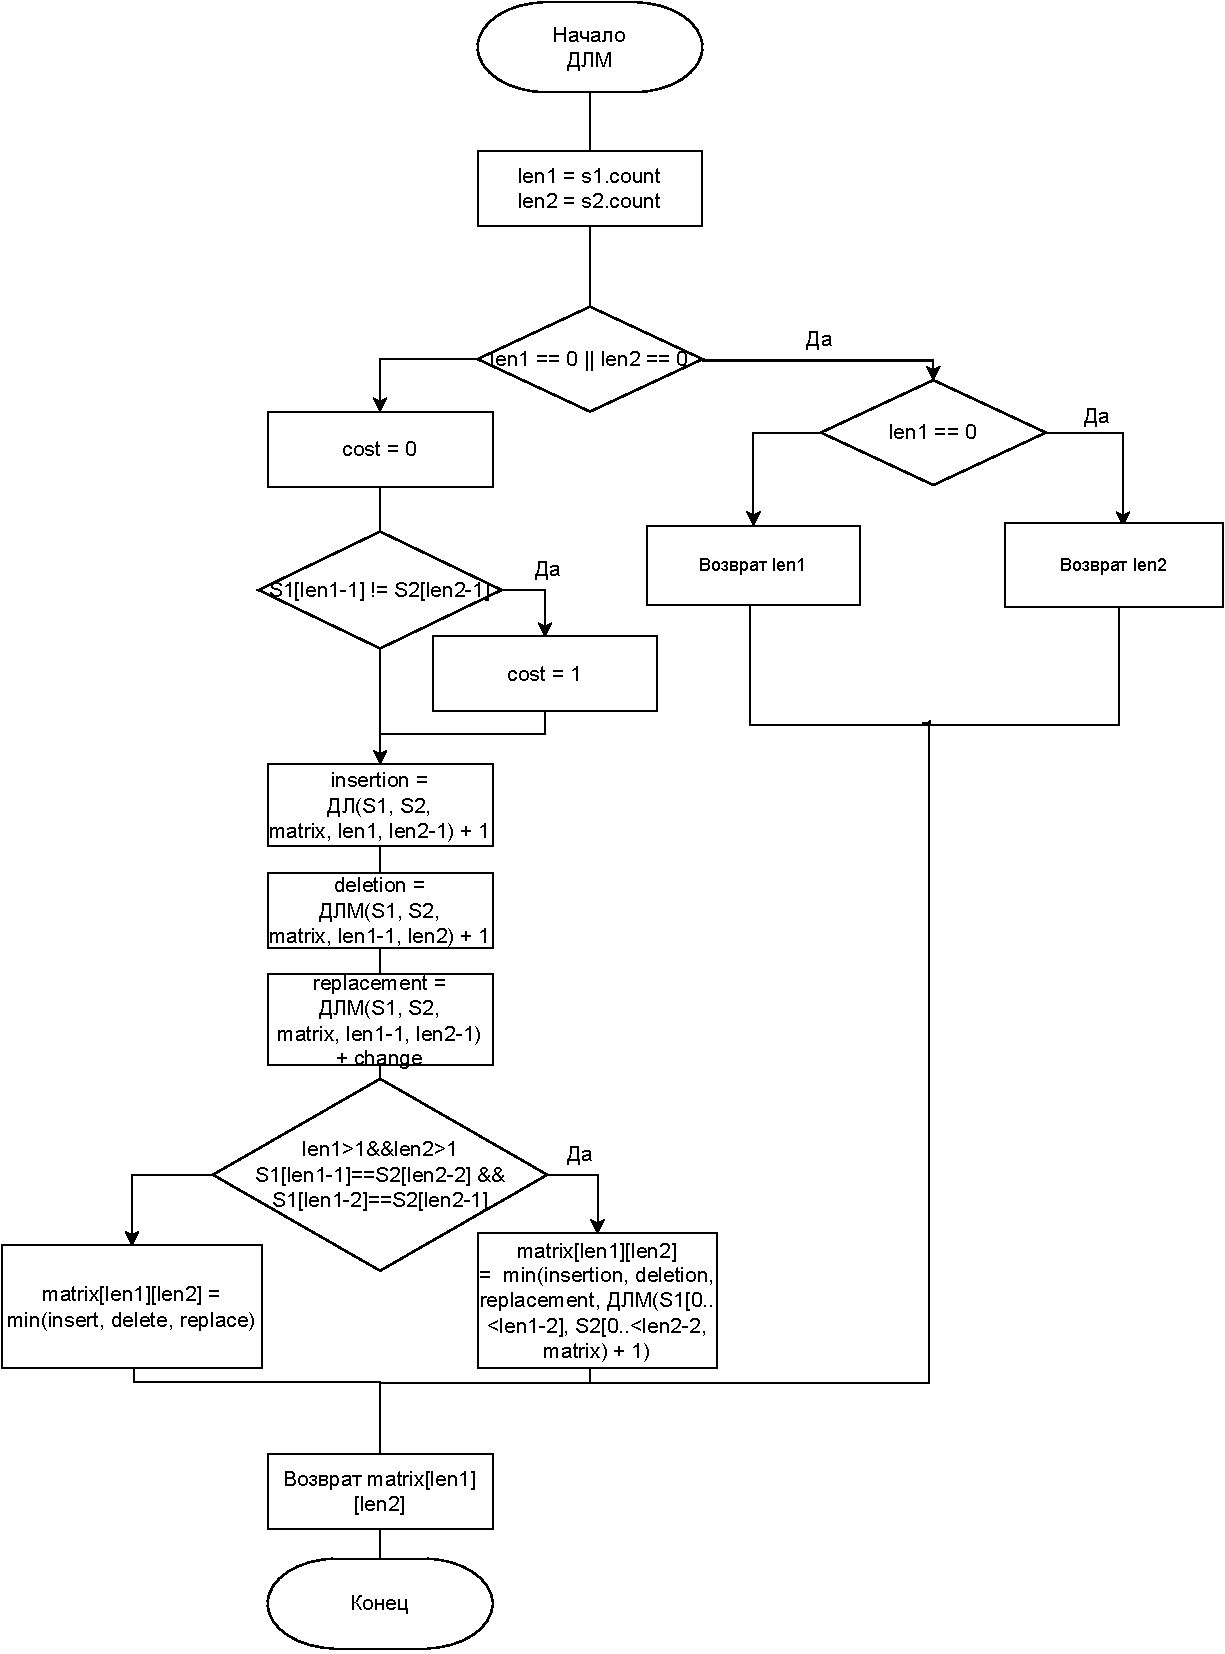
\includegraphics[height=0.8\textheight]{img/recursiveCacheDLevenshtein2.pdf}
	\caption{Схема алгоритма для рекурсивного заполнения матрицы для вычисления расстояния Дамерау~---~Левенштейна}
	\label{fig:DLrechash2}
\end{figure}

\clearpage

\section*{Вывод}

В данном разделе были представлены схемы алгоритмов для вычисления расстояний Левенштейна и Дамерау~---~Левенштейна.